\section{Modeling Objective}
\label{sec:6-1}

Estimate $P(\text{Churn} = 1 \mid \text{Customer History at Snapshot})$ on the final modeling dataset built in Chapter~\ref{ch:data-preparation} (\texttt{modeling\_dataset\_h90.parquet}). Per the Section~\ref{sec:5-6} split table, \textbf{Train} is every active row within \texttt{split=="train"} (61,415 rows of 3,905 customers, 43.0\% churn), weighted per customer by \texttt{sample\_weight} -- the training scheme chosen in Section~\ref{sec:6-scheme}; \textbf{Validation} is every row in \texttt{split=="validation"} (21,514 rows, 52.9\% churn); \textbf{Test} is every row in \texttt{split=="test"} (24,252 rows, 40.1\% churn). The three periods have noticeably different churn base rates -- a direct consequence of the seasonality already documented in Section~\ref{sec:5-4}.

Every modeling decision below is taken on validation, in a fixed order (training rows, then features, then algorithm, then hyperparameters), and test is scored once at the end. Where two candidates are close, a rule fixed in advance decides: the gap between them is bootstrapped by resampling whole \emph{customers} (500 resamples), since a customer's rows in consecutive weeks are correlated, and the simpler candidate is kept unless the 95\% interval of the gap excludes 0.

\section{Baselines}
\label{sec:6-2}

\begin{center}
\begin{tabular}{@{}p{4.2cm}p{9.9cm}@{}}
    \toprule
    Baseline & Role \\
    \midrule
    Random ranking & Reference for Lift $= 1$ and PR-AUC $=$ churn rate. \\
    Recency rule & Rank customers by recency (longest since last purchase first). A strong, business-realistic rule the models must beat. \\
    \bottomrule
\end{tabular}
\end{center}

\begin{center}
\begin{tabular}{@{}p{3.2cm}p{1.8cm}p{1.8cm}p{2.4cm}p{1.8cm}@{}}
    \toprule
    Baseline & ROC-AUC & PR-AUC & Precision@10\% & Lift@10\% \\
    \midrule
    Random & 0.495 & 0.527 & 0.535 & 1.012 \\
    Recency rule & 0.673 & 0.673 & 0.731 & 1.382 \\
    \bottomrule
\end{tabular}
\end{center}

Random ranking lands exactly where expected (ROC-AUC $\approx 0.5$, Lift $\approx 1$). The recency rule alone -- no learned parameters -- is already a credible targeting signal (Lift@10\% $= 1.38$): every model below must clear this bar to justify the added complexity of training and maintaining a classifier.

\section{Training Population}
\label{sec:6-scheme}

Section~\ref{sec:5-3} builds two ways to turn the train period into training rows: \textbf{A -- Episode}, one snapshot per customer per 90-day cooldown, unweighted (6,453 rows); and \textbf{B -- All weekly, weighted}, every active row with weight $1/n_i$ (61,415 rows). This is the first decision, since every later comparison depends on which rows are trained on. Both use Logistic Regression on the Full feature set, each with its \emph{own} regularization strength $C$ tuned over the grid 0.001, 0.003, 0.01, 0.03, 0.1, 0.3, 1, 10 and 100 -- the weights change the effective amount of regularization, so a $C$ tuned for one scheme would be unfair to the other:

\begin{center}
\begin{tabular}{@{}p{3.6cm}p{1.4cm}p{1.6cm}p{1.6cm}p{2.3cm}p{2.6cm}@{}}
    \toprule
    Scheme & Best $C$ & ROC-AUC & PR-AUC & Lift@10\% & Weekly Lift@10\% \\
    \midrule
    A -- Episode & 0.003 & 0.774 & 0.752 & 1.516 & $1.522 \pm 0.032$ \\
    B -- All weekly, weighted & 100 & 0.781 & \textbf{0.770} & \textbf{1.599} & $\mathbf{1.589 \pm 0.053}$ \\
    \bottomrule
\end{tabular}
\end{center}

B's validation PR-AUC is nearly flat for $C \geq 0.1$ (0.7696--0.7699). The customer-level bootstrap of B $-$ A gives \textbf{+0.017 PR-AUC} (95\% CI $[+0.011, +0.024]$) and \textbf{+0.079 Lift@10\%} ($[+0.025, +0.132]$), and B leads on Lift@10\% in \textbf{all 8 validation weeks}. \textbf{Scheme B is carried forward}: with only a few thousand customers, discarding over 90\% of the rows removes more signal than redundancy -- the weighted rows still see each customer at many points of their purchase cycle (just bought, overdue, about to lapse), while each customer keeps the same total influence.

\section{RFM Model}
\label{sec:6-3}

A Logistic Regression using only Recency, Frequency and Monetary features (no missing values, no imputation needed), trained on the weighted rows and scored on validation, with $C$ tuned over the same grid as Section~\ref{sec:6-scheme}:

\begin{center}
\begin{tabular}{@{}p{1.8cm}p{1.8cm}p{1.8cm}p{2.4cm}p{1.8cm}@{}}
    \toprule
    Best $C$ & ROC-AUC & PR-AUC & Precision@10\% & Lift@10\% \\
    \midrule
    100 & 0.778 & 0.769 & 0.845 & 1.598 \\
    \bottomrule
\end{tabular}
\end{center}

Already well above both baselines (Lift@10\% $1.60$ vs.\ $1.38$ for the recency rule), and nearly insensitive to $C$ (PR-AUC 0.768--0.769 across the whole grid).

\section{Extended Feature Model}
\label{sec:6-4}

Add purchase-behavior and temporal features (average order value, tenure, mean inter-purchase gap, recency relative to that gap, activity in the last 90 days). The two gap-based features are \texttt{NaN} for customers with only one occasion so far; a median imputer fit on the training rows only handles this.

\begin{center}
\begin{tabular}{@{}p{1.8cm}p{1.8cm}p{1.8cm}p{2.4cm}p{1.8cm}@{}}
    \toprule
    Best $C$ & ROC-AUC & PR-AUC & Precision@10\% & Lift@10\% \\
    \midrule
    100 & 0.781 & 0.772 & 0.847 & 1.602 \\
    \bottomrule
\end{tabular}
\end{center}

\section{Full Feature Model}
\label{sec:6-5}

Add product- and cancellation-behavior features (distinct products so far, cancellation count and value share so far). All three sets, each at its own best $C$:

\begin{center}
\begin{tabular}{@{}p{2.6cm}p{1.4cm}p{1.8cm}p{1.8cm}p{2.4cm}p{1.8cm}@{}}
    \toprule
    Feature set & Best $C$ & ROC-AUC & PR-AUC & Precision@10\% & Lift@10\% \\
    \midrule
    RFM (3) & 100 & 0.778 & 0.769 & 0.845 & 1.598 \\
    \textbf{Extended (8)} & 100 & \textbf{0.781} & \textbf{0.772} & \textbf{0.847} & \textbf{1.602} \\
    Full (11) & 100 & 0.781 & 0.770 & 0.845 & 1.599 \\
    \bottomrule
\end{tabular}
\end{center}

The three sets are within 0.004 PR-AUC of each other -- RFM alone already captures nearly all of the separable signal. The selection rule is applied to the top set, Extended:

\begin{center}
\begin{tabular}{@{}p{3.6cm}p{2.4cm}p{3.4cm}@{}}
    \toprule
    PR-AUC gap & Mean & 95\% CI \\
    \midrule
    Extended $-$ RFM & +0.0032 & $[+0.0002, +0.0063]$ \\
    Extended $-$ Full & +0.0020 & $[-0.0024, +0.0059]$ \\
    \bottomrule
\end{tabular}
\end{center}

Extended's gain over RFM is small but its interval (narrowly) excludes 0, so the rule does not fall back to RFM; Full adds nothing over Extended. \textbf{The Extended feature set is carried forward.} The earlier version of this comparison tuned $C$ only for the Full set, which made the three sets look further apart than they are.

\section{Algorithms}
\label{sec:6-6}

Compare Logistic Regression, Random Forest and XGBoost on the Extended feature set, reasonable default hyperparameters, same weighted training rows and validation split:

\begin{center}
\begin{tabular}{@{}p{3.6cm}p{1.8cm}p{1.8cm}p{2.4cm}p{1.8cm}@{}}
    \toprule
    Algorithm & ROC-AUC & PR-AUC & Precision@10\% & Lift@10\% \\
    \midrule
    \textbf{Logistic Regression} & \textbf{0.781} & \textbf{0.772} & \textbf{0.846} & \textbf{1.600} \\
    Random Forest & 0.770 & 0.755 & 0.836 & 1.581 \\
    XGBoost & 0.756 & 0.745 & 0.827 & 1.564 \\
    \bottomrule
\end{tabular}
\end{center}

Logistic Regression wins on every metric, even with ten times more training rows than the episode scheme provides. The weekly rows add correlated views of the same 3,905 customers rather than new customers, so the tree ensembles still have little room to find reliable non-linear splits; the relationships in these features are close to monotonic, which suits the linear model. \textbf{Logistic Regression on the Extended feature set is carried forward} to hyperparameter tuning.

\section{Hyperparameter Tuning}
\label{sec:6-7}

Tune on the validation period while preserving temporal separation (fit on train, compare on validation -- not a cross-validated search, which would break the temporal structure):

\begin{center}
\begin{tabular}{@{}p{1.8cm}p{1.8cm}p{1.8cm}p{2.4cm}p{3.6cm}@{}}
    \toprule
    $C$ & ROC-AUC & PR-AUC & Lift@10\% & PR-AUC gap to best (95\% CI) \\
    \midrule
    0.001 & 0.775 & 0.763 & 1.586 & $+0.0084$ $[+0.0046, +0.0122]$ \\
    0.003 & 0.777 & 0.767 & 1.598 & $+0.0048$ $[+0.0017, +0.0079]$ \\
    \textbf{0.01} & \textbf{0.780} & \textbf{0.770} & \textbf{1.603} & $\mathbf{+0.0017}$ $\mathbf{[-0.0003, +0.0037]}$ \\
    0.03 & 0.781 & 0.771 & 1.602 & $+0.0004$ $[-0.0007, +0.0015]$ \\
    0.1 & 0.781 & 0.772 & 1.600 & $+0.0001$ $[-0.0004, +0.0006]$ \\
    1.0 & 0.781 & 0.772 & 1.600 & $+0.0001$ $[-0.0001, +0.0002]$ \\
    100 & 0.781 & 0.772 & 1.602 & -- (best) \\
    \bottomrule
\end{tabular}
\end{center}

Validation PR-AUC barely moves above $C = 0.01$, but the coefficients do: frequency, monetary value and average order value are strongly correlated ($\log$ monetary $\approx$ $\log$ frequency $+$ $\log$ order value), and with weak regularization they trade off against each other -- at $C = 100$ on the final training pool, the frequency coefficient turns \emph{positive} (more purchases $\Rightarrow$ more churn, conditionally) while monetary and order value inflate in opposite directions. The ranking barely changes, but no single coefficient can be read on its own. The same parsimony rule as Section~\ref{sec:6-5} therefore applies: \textbf{take the strongest regularization whose PR-AUC gap to the best $C$ has an interval that includes 0} -- here $C = 0.01$, where every coefficient keeps its intuitive sign (Section~\ref{sec:6-9}).

The final model is then refit on \textbf{every labelable active row from the first train date to the last validation date} -- 120,376 rows of 4,571 customers, with $1/n_i$ recomputed over this longer window -- and evaluated \textbf{once} on test:

\begin{center}
\begin{tabular}{@{}p{1.8cm}p{1.8cm}p{2.4cm}p{1.8cm}p{1.8cm}p{2.8cm}@{}}
    \toprule
    ROC-AUC & PR-AUC & Precision@10\% & Lift@10\% & Gain@10\% & Weekly Lift@10\% \\
    \midrule
    0.759 & 0.654 & 0.757 & 1.889 & 0.189 & $1.888 \pm 0.061$ \\
    \bottomrule
\end{tabular}
\end{center}

ROC-AUC on test (0.759) is close to validation (0.780) -- no meaningful overfitting from the refit. PR-AUC is lower on test (0.654 vs.\ 0.770) because the test period's churn rate is lower (40.1\% vs.\ 52.9\% validation) and PR-AUC's baseline moves with the base rate; Lift@10\% (which normalizes for base rate) is \emph{higher} on test (1.89 vs.\ 1.60 on validation), confirming the model's ranking ability holds up out of sample.

\textbf{For reference only -- not used for any decision.} The same configuration refit on the episode-sampled rows of the same window (scheme A, 12,019 rows) reaches ROC-AUC 0.764, PR-AUC 0.656 and weekly Lift@10\% $1.883 \pm 0.062$ on test -- practically the same as the final model. Most of Section~\ref{sec:6-scheme}'s validation gap therefore came from scheme A's small training sample (6,453 rows); once both schemes are refit on twice the data, the weighted scheme keeps only a marginal edge. It is still the scheme chosen by the validation protocol, and it costs nothing extra to train.

\section{Model Selection}
\label{sec:6-8}

The final model is \textbf{Logistic Regression, Extended feature set (8 features), $C = 0.01$, trained on every weekly active row with per-customer weight $1/n_i$}, refit on train+validation (120,376 rows) and evaluated once on test. Each choice was made on validation by the rules above: the weighted scheme beats episode sampling with an interval that excludes 0 (Section~\ref{sec:6-scheme}); Extended is the best feature set and is not tied with RFM (Section~\ref{sec:6-5}); Logistic Regression beats both tree ensembles (Section~\ref{sec:6-6}); and $C = 0.01$ is the strongest regularization statistically tied with the best (Section~\ref{sec:6-7}). On test, the final model reaches \textbf{Lift@10\% $= 1.89$} and \textbf{Gain@10\% $= 0.189$} -- targeting the top 10\% of ranked customers each week would reach churners at nearly twice the rate of untargeted outreach, capturing 18.9\% of all churners in that 10\% of the population.

Compared with the earlier version of this chapter (episode-sampled rows, Full features, $C = 0.01$: test ROC-AUC 0.765, PR-AUC 0.658), test performance is essentially unchanged; what changed is that every choice now follows from a fair validation comparison, and the final coefficients are interpretable.

\section{Model Interpretability}
\label{sec:6-9}

SHAP values for the final refit model (\texttt{LinearExplainer}, computed on a sample of 1,000 test rows):

\begin{center}
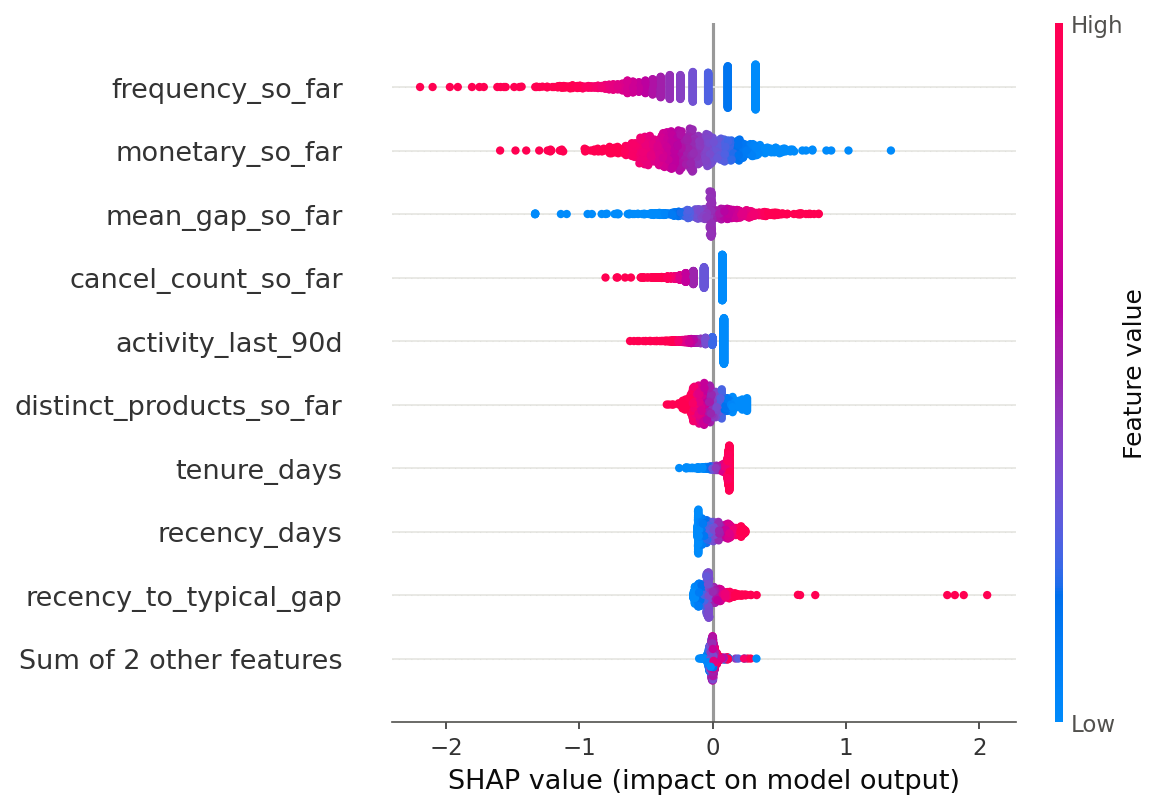
\includegraphics[width=0.85\textwidth]{figures/ch8_shap_summary.png}
\end{center}

By mean absolute SHAP value, the most influential features are \texttt{frequency\_so\_far} and \texttt{monetary\_so\_far} (the two RFM features driving most of the model's separating power, consistent with Sections~\ref{sec:6-3}--\ref{sec:6-5}), followed by \texttt{recency\_days}, the mean inter-purchase gap and \texttt{activity\_last\_90d}. Every direction is the intuitive one: more purchases, more spend and more recent activity push the prediction toward \emph{not} churning, while a longer time since the last purchase and a longer typical gap between purchases push toward churning. \texttt{recency\_to\_typical\_gap} is near zero for most customers but shows the widest spread at its extreme values (customers far more overdue than their own normal rhythm), the clearest individual red flag in the tail. Two features carry little weight once the others are known: average order value (its information is already in monetary value divided by frequency) and tenure, which pushes slightly toward churning once frequency is held fixed (a long-standing customer with few purchases is a slow buyer). These signs depend on the regularization chosen in Section~\ref{sec:6-7}: with weak regularization, the correlated frequency, monetary and order-value coefficients trade off and some flip sign. \textbf{These are associations the model has learned, not causal effects} (Chapter~\ref{ch:evaluation}).
